%% Results narrative. Numbers are macros from tables/numbers.tex; re-check every qualitative
%% sentence (marked %CHECK) after the final full run, since directions can change.

\subsection{Clean detection}
Table~\ref{tab:clean} lists clean performance. LightGBM, the EMBER reference model, reaches \LgbmAcc\% accuracy and the standard MLP \MlpAcc\%. Most certifiable models cost little or no clean accuracy: the symmetric CROWN-IBP network reaches \CrownSymAcc\% (standard network of the same size: \StdAccSmall\%). The clearest cost is group ablation with single-group views ($k=1$, \AblOneCleanAcc\%), which loses more than one point against the standard MLP; larger keep sizes recover most of it ($k=3$: \AblThreeCleanAcc\%). %CHECK

\begin{table}[t]\centering\small
\caption{Clean test performance (mean $\pm$ std over \NSeeds{} \SeedsNoun{}).}\label{tab:clean}
\resizebox{\linewidth}{!}{\begin{tabular}{lccccc}
\toprule
Model & Acc. (\%) & F1 (\%) & TPR (\%) & FPR (\%) & AUC \\
\midrule
LightGBM (EMBER baseline) & 99.53$\pm$0.05 & 99.45$\pm$0.06 & 99.39$\pm$0.11 & 0.36$\pm$0.01 & 0.9998$\pm$0.0001 \\
MLP (standard) & 99.23$\pm$0.17 & 99.10$\pm$0.20 & 99.21$\pm$0.20 & 0.74$\pm$0.15 & 0.9985$\pm$0.0004 \\
MLP + PGD-AT & 99.34$\pm$0.11 & 99.22$\pm$0.13 & 99.27$\pm$0.15 & 0.61$\pm$0.09 & 0.9994$\pm$0.0003 \\
Group ablation, $k$=1 & 97.88$\pm$0.19 & 97.48$\pm$0.23 & 95.92$\pm$0.27 & 0.66$\pm$0.13 & 0.9972$\pm$0.0007 \\
Group ablation, $k$=2 & 98.77$\pm$0.05 & 98.56$\pm$0.06 & 98.40$\pm$0.18 & 0.95$\pm$0.12 & 0.9991$\pm$0.0002 \\
Group ablation, $k$=3 & 99.24$\pm$0.11 & 99.11$\pm$0.13 & 99.04$\pm$0.07 & 0.61$\pm$0.14 & 0.9994$\pm$0.0004 \\
IBP ($\epsilon$=0.05) & 99.37$\pm$0.16 & 99.26$\pm$0.19 & 99.35$\pm$0.16 & 0.61$\pm$0.17 & 0.9989$\pm$0.0004 \\
CROWN-IBP ($\epsilon$=0.05) & 99.33$\pm$0.17 & 99.21$\pm$0.20 & 99.28$\pm$0.24 & 0.64$\pm$0.13 & 0.9990$\pm$0.0004 \\
CROWN-IBP (asym.) ($\epsilon$=0.05) & 98.71$\pm$0.08 & 98.51$\pm$0.09 & 99.70$\pm$0.10 & 2.02$\pm$0.11 & 0.9950$\pm$0.0008 \\
\bottomrule
\end{tabular}}
\end{table}

\subsection{C1: constrained attacks}
Figure~\ref{fig:attacks} and Table~\ref{tab:attacks} show the malware detection rate that survives FGSM and PGD. Restricting the attacker to the reachable region weakens every attack: at $\epsilon=\AtkEps$, PGD evades the standard MLP on \MlpPgdCon\% of malware under constraints versus \MlpPgdUnc\% without them, so unconstrained evaluations overstate the threat. PGD adversarial training at $\epsilon=0.1$ reduces constrained evasion at the same budget to \AtPgdCon\%; its protection degrades beyond the training budget and is gone by $\epsilon=0.5$ (Table~\ref{tab:attacks}). %CHECK The group-transplant attack is far more damaging: copying a single feature group from a benign file evades the standard MLP on \MlpGroupEvadeOne\% of attacked malware (Fig.~\ref{fig:group}, grey). This motivates certificates against group-level edits rather than small norm balls.

\begin{figure}[t]\centering
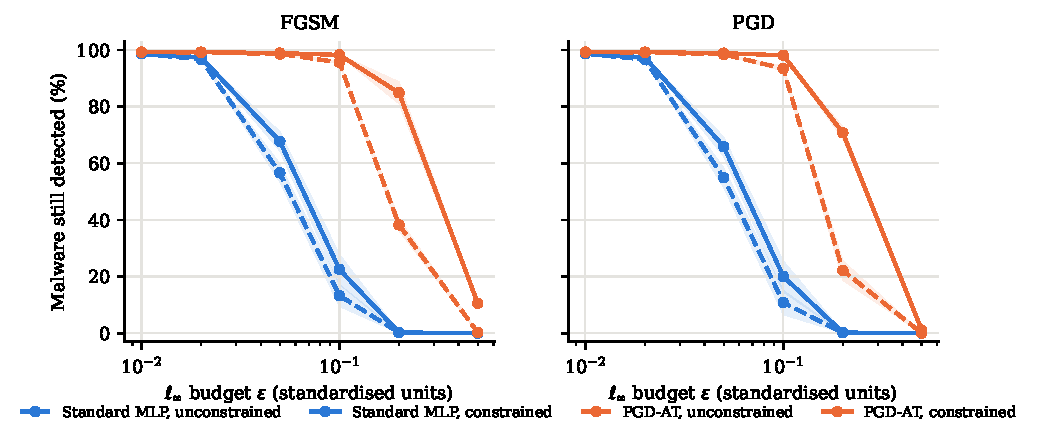
\includegraphics[width=\linewidth]{figures/fig_attacks.pdf}
\caption{Malware still detected under FGSM and PGD as the $\ell_\infty$ budget grows. Dashed: unconstrained attacker; solid: constrained (C1) attacker.}\label{fig:attacks}
\end{figure}

\begin{table}[t]\centering\small
\caption{Malware detection rate (\%) under PGD.}\label{tab:attacks}
\resizebox{\linewidth}{!}{\begin{tabular}{lrrrr}
\toprule
Detector & $r=0$ & $r=1$ & $r=2$ & $r=3$ \\
\midrule
LightGBM (all features) & 88.5 & 0.0 & 0.0 & 0.0 \\
LightGBM, monotonic & 88.6 & 0.0 & 0.0 & 0.0 \\
MLP 2381--512--256--2 & 83.3 & 0.2 & 0.0 & 0.0 \\
MLP 2381--256--256--2 & 82.3 & 0.2 & 0.0 & 0.0 \\
PGD-AT on $B_\epsilon$ & 83.5 & 0.3 & 0.0 & 0.0 \\
Group ablation, MLP views, main & 74.1 & 49.9 & 0.0 & 0.0 \\
Group ablation, MLP views, second & 69.8 & 26.1 & 0.0 & 0.0 \\
Group ablation, MLP views, EMBER groups & 60.8 & 0.0 & 0.0 & 0.0 \\
Group ablation, LightGBM views, main & 83.4 & 62.6 & 0.0 & 0.0 \\
Group ablation, LightGBM views, second & 78.8 & 37.0 & 0.0 & 0.0 \\
CROWN-IBP, uniform ball & 82.3 & 0.0 & 0.0 & 0.0 \\
CROWN-IBP, constrained box & 84.5 & 0.2 & 0.0 & 0.0 \\
CROWN-IBP, edit-aware & 81.5 & 2.0 & 0.1 & 0.0 \\
Giri et al., re-implementation & 82.3 & 0.7 & 0.0 & 0.0 \\
\bottomrule
\end{tabular}
% malware detected (%) under the group-transplant attack in the main partition's groups; mean over 5 seeds; 500 malware, 10 donors}
\end{table}

\subsection{C2a: feature-group ablation certificates}
Table~\ref{tab:group} and Fig.~\ref{fig:group} report certified detection as a function of the number $r$ of modified groups. Keep-size $k$ trades clean accuracy for certifiable $r$: with $k=1$ (nine single-group views) the detector certifies \AblOneCertR\% of malware against any change to one group and \AblOneCertRtwo\% against two, at \AblOneCleanAcc\% clean accuracy; $k=2$ certifies \AblTwoCertR\% at $r=1$ with \AblTwoCleanAcc\% accuracy; $k=3$ certifies \AblThreeCertR\% at $r=1$ with \AblThreeCleanAcc\% accuracy but nothing at $r\geq2$, as Theorem~\ref{thm:abl} predicts ($2\Delta_2=98$ exceeds the 84 views). The greedy group-transplant attack against the $k=1$ detector leaves \AblOneEmpR\% and \AblOneEmpRtwo\% of malware detected at $r=1,2$, close to the certified values, so the certificate is nearly tight. Across all runs the attack never evaded a certified sample (\AblViolations{} violations), as required by soundness.

\begin{figure}[t]\centering
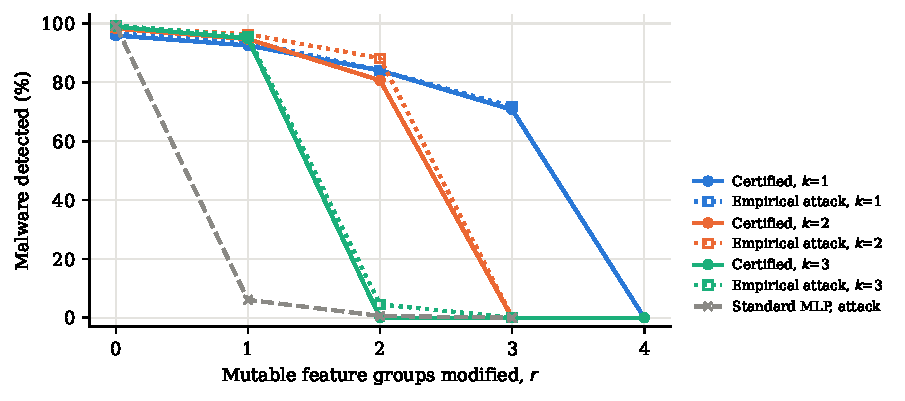
\includegraphics[width=0.88\linewidth]{figures/fig_group_cert.pdf}
\caption{Certified malware detection (solid) and detection under the group-transplant attack (dotted) versus the number of modified groups. Grey: undefended MLP.}\label{fig:group}
\end{figure}

\begin{table}[t]\centering\small
\caption{Certified malware detection (\%) of group-ablation smoothing against $r$ modified groups.}\label{tab:group}
\resizebox{\linewidth}{!}{\begin{tabular}{lrrrrrrrr}
\toprule
 & \multicolumn{3}{c}{$r$ needed} & \multicolumn{5}{c}{Certified detection (\%)} \\
\cmidrule(lr){2-4}\cmidrule(lr){5-9}
Edit type & main & second & EMBER & main, MLP & main, LightGBM & second, MLP & second, LightGBM & EMBER, MLP \\
\midrule
E1 overlay append & 1 & 1 & 4 & 36.6 & 55.1 & 57.7 & 64.4 & 0.0 \\
E2 string padding & 1 & 1 & 4 & 36.6 & 55.1 & 57.7 & 64.4 & 0.0 \\
E3 section injection & 2 & 2 & 6 & 0.0 & 0.0 & 42.1 & 52.4 & 0.0 \\
E4 import addition & 3 & 3 & 7 & 0.0 & 0.0 & 18.2 & 32.2 & 0.0 \\
E5 timestamp & 1 & 1 & 3 & 36.6 & 55.1 & 57.7 & 64.4 & 27.0 \\
E6 section renaming & 2 & 2 & 4 & 0.0 & 0.0 & 42.1 & 52.4 & 0.0 \\
E7 checksum, DOS header & 1 & 1 & 3 & 36.6 & 55.1 & 57.7 & 64.4 & 27.0 \\
E8 signature/debug strip & 2 & 3 & 6 & 0.0 & 0.0 & 18.2 & 32.2 & 0.0 \\
E10 header versions & 1 & 2 & 3 & 36.6 & 55.1 & 42.1 & 52.4 & 27.0 \\
\midrule
Mean over the nine types &  &  &  & 20.3\,$\pm$\,3.9 & 30.6\,$\pm$\,5.2 & 43.7\,$\pm$\,5.2 & 53.2\,$\pm$\,8.6 & 9.0\,$\pm$\,2.3 \\
Clean accuracy &  &  &  & 88.5\,$\pm$\,3.3 & 92.8\,$\pm$\,2.4 & 86.0\,$\pm$\,3.6 & 90.8\,$\pm$\,5.1 & 83.0\,$\pm$\,2.7 \\
Views; largest certifiable $r$ &  &  &  & 10; 1 & 10; 1 & 7; 3 & 7; 3 & 9; 4 \\
\bottomrule
\end{tabular}
% family split, 5 seeds; main = aligned5 k=2, second = aligned7 k=1, EMBER = 9 groups k=1}
\end{table}

\subsection{C2b: randomized smoothing}
Contrary to the common assumption that smoothing collapses clean accuracy on PE features, Gaussian smoothing in standardised feature space keeps clean accuracy high: at $\sigma=\RsSigmaMax$ it is \RsIsoAccMax\% (isotropic) and \RsSubAccMax\% (subspace) on the \NCertPoints{} certified test points. %CHECK
Restricting noise to the mutable subspace gives at most a small change (\RsSubHalf\% vs.\ \RsIsoHalf\% certified at $R=0.5$, $\sigma=\RsSigma$), because \MutablePct\% of the features are mutable: the subspace removes little noise. %CHECK
The sharp drop of each curve in Fig.~\ref{fig:smoothing} is the sampling ceiling $\sigma\Phi^{-1}(\underline{p_A})$ for $n=\NCert$ samples, not a property of the classifier. Smoothing radii in standardised $\ell_2$ units are also hard to relate to real edits, which is why we treat this certificate as a baseline rather than a headline result.

\begin{figure}[t]\centering
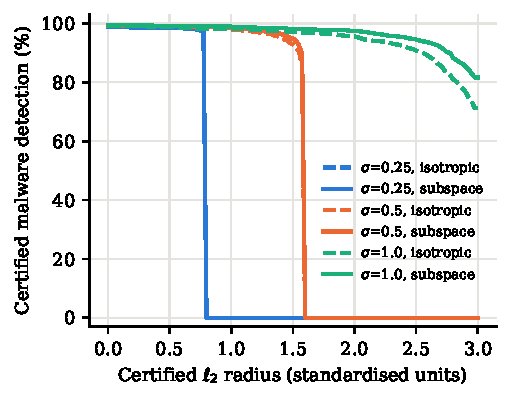
\includegraphics[width=0.62\linewidth]{figures/fig_smoothing.pdf}
\caption{Certified malware detection of Gaussian smoothing versus $\ell_2$ radius; dashed: noise on all features, solid: noise only on mutable features.}\label{fig:smoothing}
\end{figure}

\begin{table}[t]\centering\small
\caption{Randomized smoothing: clean accuracy and certified malware detection (\%) at several radii.}\label{tab:smoothing}
\resizebox{\linewidth}{!}{\begin{tabular}{llccccc}
\toprule
$\sigma$ & Noise & Clean acc. (\%) & $R\geq$0.0 & $R\geq$0.25 & $R\geq$0.5 & $R\geq$1.0 \\
\midrule
0.25 & isotropic & 99.1$\pm$0.4 & 99.1 & 99.0 & 98.6 & 0.0 \\
0.25 & subspace & 99.1$\pm$0.3 & 98.9 & 98.7 & 98.5 & 0.0 \\
0.5 & isotropic & 99.2$\pm$0.2 & 99.4 & 99.3 & 99.0 & 98.0 \\
0.5 & subspace & 99.1$\pm$0.3 & 99.2 & 99.1 & 99.1 & 98.4 \\
1.0 & isotropic & 99.3$\pm$0.4 & 99.3 & 99.2 & 98.9 & 98.0 \\
1.0 & subspace & 99.4$\pm$0.2 & 99.4 & 99.3 & 99.3 & 98.9 \\
\bottomrule
\end{tabular}}
\end{table}

\subsection{C3: constraint-aware certified training}\label{sec:ct}
Figure~\ref{fig:ct} and Table~\ref{tab:ct} show certified malware detection under the constrained $\ell_\infty$ threat. Standard and PGD-trained networks are rarely certifiable at the training budget ($\epsilon=\TrainEps$: \StdCert\% and \PgdAtCert\%), although PGD-AT resists the attack empirically. IBP and CROWN-IBP training raise certified detection to \IbpCert\% and \CrownSymCert\% at no measurable cost in clean accuracy. Bounding over the constrained box instead of the full ball certifies more samples, and the gain grows with the budget: \CrownSymCert\% vs.\ \CrownSymCertUnc\% at $\epsilon=\TrainEps$ and \CrownSymCertTen\% vs.\ \CrownSymCertTenUnc\% at $\epsilon=0.1$. %CHECK
Asymmetric training does not pay off. At $\epsilon=\TrainEps$ it certifies \CrownAsymCert$\pm$\CrownAsymCertStd\% of malware versus \CrownSymCert$\pm$\CrownSymCertStd\% for symmetric CROWN-IBP, a gain within seed-to-seed variation (though positive \AsymGainSeeds); at $\epsilon=0.1$ it certifies less (\CrownAsymCertTen$\pm$\CrownAsymCertTenStd\% vs.\ \CrownSymCertTen$\pm$\CrownSymCertTenStd\%, lower \AsymLossTenSeeds); and it raises the false-positive rate from \CrownSymFpr\% to \CrownAsymFpr\%: making only malware robust pushes the decision boundary into benign territory. In deployment, where false positives are costly, symmetric CROWN-IBP is the better operating point. %CHECK
No sample certified by bound propagation was ever evaded by PGD (\CTViolations{} violations).

\begin{figure}[t]\centering
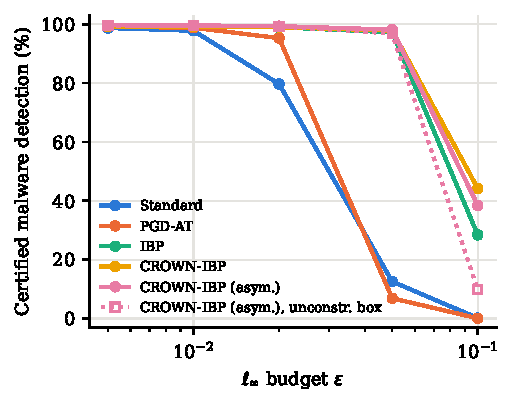
\includegraphics[width=0.62\linewidth]{figures/fig_certified_training.pdf}
\caption{Certified malware detection versus $\ell_\infty$ budget (constrained box), for networks with the same 2381--256--256--2 architecture. Dotted: asymmetric CROWN-IBP certified over the unconstrained box.}\label{fig:ct}
\end{figure}

\begin{table}[t]\centering\small
\caption{Certified malware detection (\%) under the constrained $\ell_\infty$ threat; last column: certified samples evaded by PGD (must be 0).}\label{tab:ct}
\resizebox{\linewidth}{!}{\begin{tabular}{lrrrrrrrr}
\toprule
 & & & \multicolumn{5}{c}{Certified over $T_f(1)$ (\%)} & \\
\cmidrule(lr){4-8}
CROWN-IBP training & Acc. & FPR & content & section & import & strip & mean & $B_\epsilon$, $\epsilon=0.05$ \\
\midrule
Standard MLP & 91.7 & 0.6 & 0.0 & 0.0 & 0.0 & 0.0 & 0.0\,$\pm$\,0.0 & 3.6 \\
PGD-AT & 92.7 & 0.4 & 0.0 & 0.0 & 0.0 & 0.0 & 0.0\,$\pm$\,0.0 & 1.7 \\
Uniform ball, $\epsilon=0.1$ (tuned) & 92.2 & 0.4 & 0.0 & 0.0 & 0.0 & 0.1 & 0.0\,$\pm$\,0.0 & 72.6 \\
Constrained box, $\epsilon=0.1$ & 93.0 & 0.4 & 0.0 & 0.0 & 0.0 & 0.0 & 0.0\,$\pm$\,0.0 & 73.1 \\
Edit-aware & 91.4 & 1.2 & 40.7 & 66.8 & 40.2 & 76.3 & 56.0\,$\pm$\,7.0 & 71.0 \\
Uniform ball, $\epsilon=1$ (sweep) & 89.9 & 6.5 & 72.5 & 32.6 & 0.0 & 84.2 & 47.3\,$\pm$\,17.6 & -- \\
\bottomrule
\end{tabular}
% family split, 5 seeds (sweep row: results_eps_sweep); networks 2381--256--256--2}
\end{table}

\subsection{Per-category robustness}
Figure~\ref{fig:cat} breaks certified detection down by malware category, averaged over the \NSeeds{} seeds' test splits. Large categories (trojan, worm, backdoor) are certified at high rates by every method, trojans being the lowest of the three, while bound-propagation certificates are more uniform across categories than the group certificate. The group certificate is lowest on file-infecting viruses, plausibly because an infected host is mostly benign content so few single-group views vote malware. This observation remains tentative: each test split holds fewer than ten viruses, and even across all seeds the number of distinct viruses tested (shown in the figure) is small. Information stealers and viruses are the two weakest categories for every method. %CHECK

\begin{figure}[t]\centering
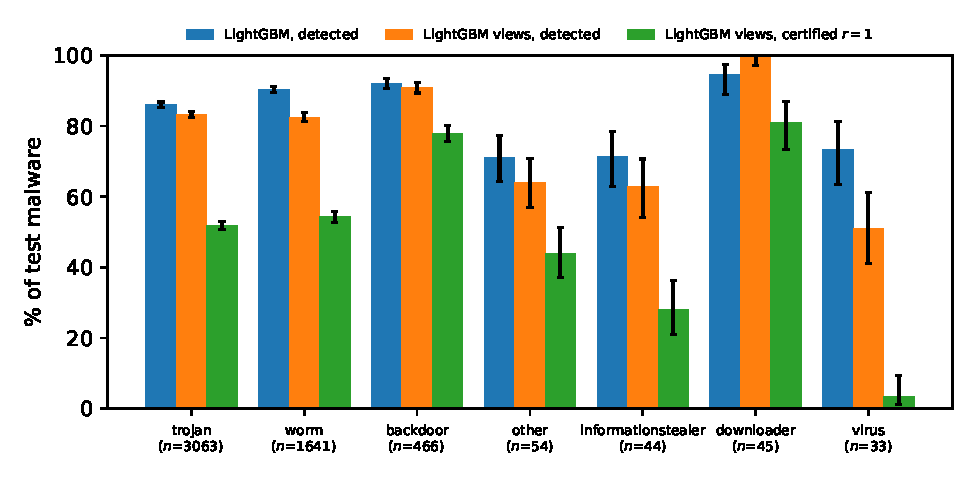
\includegraphics[width=0.72\linewidth]{figures/fig_per_category.pdf}
\caption{Certified malware detection (\%) per category, averaged over the \NSeeds{} seeds' test splits ($n$ = distinct test files across all seeds). Not shown, for having fewer than three test samples per seed on average: \HiddenCats.}\label{fig:cat}
\end{figure}

\subsection{Robustness under temporal drift}\label{sec:temporal}
Following the temporal-split principle of \citet{pendlebury2019tesseract}, in which every training file precedes every test file, we also train on files up to \TmpTrainEnd{} and test on the later window \TmpTestStart{} to \TmpTestEnd{} (Tables~\ref{tab:temporal-clean} and~\ref{tab:temporal-cert}). We measure drift by malware detection (TPR) rather than accuracy: the false-positive rate drops for \TmpFprDropModels{} on the temporal window (standard MLP: \TmpMlpFprRand\% to \TmpMlpFprTemp\%; CROWN-IBP: \TmpCrownFprRand\% to \TmpCrownFprTemp\%), which inflates accuracy, and the temporal test window holds a \TmpMalShareCmp{} share of malware (\TmpMalShareTemp\% vs.\ \TmpMalShareRand\%), which changes accuracy as well. For CROWN-IBP, clean detection falls by \TmpCrownTprDrop$\pm$\TmpCrownTprDropStd{} points and certified detection at $\epsilon=\TmpCertEps$ by \TmpCrownCertDrop$\pm$\TmpCrownCertDropStd{}, roughly \TmpCrownDropRatioInt{} times as much; the gap is \TmpCrownGapRatio{} times their combined standard deviation. For group ablation ($k=1$), clean detection falls by \TmpAblTprDrop$\pm$\TmpAblTprDropStd{} points and certified detection at $r=1$ by \TmpAblCertDrop$\pm$\TmpAblCertDropStd{}; the gap of \TmpAblGap{} points is about one combined standard deviation (\TmpAblDropStd{}), so we do not claim it as significant. Across keep sizes, $k=3$ drifts less than $k=1$ in both clean and certified detection (\TmpAblThreeTprDrop$\pm$\TmpAblThreeTprDropStd{} vs.\ \TmpAblTprDrop$\pm$\TmpAblTprDropStd{} points of clean detection; \TmpAblThreeCertDrop$\pm$\TmpAblThreeCertDropStd{} vs.\ \TmpAblCertDrop$\pm$\TmpAblCertDropStd{} points of certified detection at $r=1$); $k=2$ lies between on average, with high variance in certified detection (\TmpAblTwoCertDrop$\pm$\TmpAblTwoCertDropStd{} points). \TmpCrownVsMlpSentence{} \TmpCrownVsMlpAccSentence{} %CHECK

\begin{table}[t]\centering\small
\caption{Clean test performance (\%) under the random and the temporal split (mean $\pm$ std over \NSeeds{} \SeedsNoun{}). The temporal split uses one fixed test window (\TmpTestStart{} to \TmpTestEnd{}), so its $\pm$ reflects training randomness only; values without $\pm$ are identical across seeds.}\label{tab:temporal-clean}
\resizebox{\linewidth}{!}{\begin{tabular}{lcccccc}
\toprule
 & \multicolumn{3}{c}{Random split} & \multicolumn{3}{c}{Temporal split} \\
\cmidrule(lr){2-4}\cmidrule(lr){5-7}
Model & Acc. & TPR & FPR & Acc. & TPR & FPR \\
\midrule
LightGBM & 99.53$\pm$0.05 & 99.39$\pm$0.11 & 0.36$\pm$0.01 & 99.52 & 99.11 & 0.07 \\
MLP (standard) & 99.23$\pm$0.17 & 99.21$\pm$0.20 & 0.74$\pm$0.15 & 97.43$\pm$0.40 & 95.09$\pm$0.82 & 0.19$\pm$0.03 \\
MLP + PGD-AT & 99.34$\pm$0.11 & 99.27$\pm$0.15 & 0.61$\pm$0.09 & 98.96$\pm$0.09 & 98.03$\pm$0.18 & 0.09$\pm$0.02 \\
Group ablation, $k$=1 & 97.88$\pm$0.19 & 95.92$\pm$0.27 & 0.66$\pm$0.13 & 90.06$\pm$1.55 & 80.36$\pm$3.06 & 0.08$\pm$0.02 \\
Group ablation, $k$=2 & 98.77$\pm$0.05 & 98.40$\pm$0.18 & 0.95$\pm$0.12 & 95.04$\pm$0.03 & 90.28$\pm$0.05 & 0.12$\pm$0.02 \\
Group ablation, $k$=3 & 99.24$\pm$0.11 & 99.04$\pm$0.07 & 0.61$\pm$0.14 & 98.44$\pm$0.04 & 96.99$\pm$0.07 & 0.09$\pm$0.02 \\
CROWN-IBP ($\epsilon$=0.05) & 99.33$\pm$0.17 & 99.28$\pm$0.24 & 0.64$\pm$0.13 & 98.64$\pm$0.08 & 97.35$\pm$0.17 & 0.04$\pm$0.02 \\
\bottomrule
\end{tabular}}
\end{table}

\begin{table}[t]\centering\small
\caption{Certified malware detection (\%) under the random and the temporal split (mean $\pm$ std over \NSeeds{} \SeedsNoun{}), and its drop (random minus temporal), whose $\pm$ combines the standard deviations of both splits. In the text, differences between drops are judged against the combined seed-to-seed standard deviation, which is conservative (assumes independence).}\label{tab:temporal-cert}
\resizebox{\linewidth}{!}{\begin{tabular}{llccc}
\toprule
Model & Certificate & Random split & Temporal split & Drop \\
\midrule
Group ablation, $k$=1 & $r$=1 & 92.5$\pm$0.7 & 73.2$\pm$0.9 & 19.3$\pm$1.2 \\
Group ablation, $k$=1 & $r$=2 & 84.0$\pm$0.4 & 61.1$\pm$2.9 & 22.9$\pm$2.9 \\
Group ablation, $k$=2 & $r$=1 & 94.7$\pm$0.2 & 77.2$\pm$4.1 & 17.5$\pm$4.1 \\
Group ablation, $k$=2 & $r$=2 & 80.7$\pm$0.4 & 56.2$\pm$0.9 & 24.5$\pm$1.0 \\
Group ablation, $k$=3 & $r$=1 & 94.9$\pm$0.1 & 80.6$\pm$1.7 & 14.3$\pm$1.7 \\
Group ablation, $k$=3 & $r$=2 & 0.0 & 0.0 & 0.0 \\
CROWN-IBP & $\epsilon$=0.05 & 97.9$\pm$0.2 & 88.6$\pm$1.8 & 9.3$\pm$1.8 \\
\bottomrule
\end{tabular}}
\end{table}
